\documentclass[12pt]{article}

\usepackage{tabularx}
\usepackage[table]{xcolor}
\usepackage{multirow}

\newcolumntype{C}{ >{\centering\arraybackslash} m{4cm} }
\newcolumntype{E}{ >{\centering\arraybackslash} m{11cm} }
\newcolumntype{D}{ >{\centering\arraybackslash} m{3cm} }
\newcolumntype{F}{ >{\centering\arraybackslash} m{1cm} }
\newcolumntype{G}{ >{\centering\arraybackslash} m{2cm} }
\newcolumntype{H}{ >{\centering\arraybackslash} m{8cm} }
\newcolumntype{K}{ >{\centering\arraybackslash} m{7cm} }
\newcolumntype{Y}{ >{\centering\arraybackslash} m{10cm} }


\usepackage{color}
\usepackage{xcolor}

\usepackage[margin=1.1in,footskip=.25in]{geometry}

\usepackage{listings}

\lstdefinestyle{mystyle2}{
    basicstyle=\ttfamily\small,
    breakatwhitespace=false,         
    breaklines=true,                 
    captionpos=b,                    
    keepspaces=true,                             
    showspaces=false,                
    showstringspaces=false,
    showtabs=false,                  
    tabsize=3,
}

\lstset{style=mystyle2}

\usepackage{amsmath, amssymb}
\usepackage{mathtools}
\DeclarePairedDelimiter{\ceil}{\lceil}{\rceil}
\DeclarePairedDelimiter\floor{\lfloor}{\rfloor}

\usepackage[most]{tcolorbox}

\tcbset{
    frame code={}
    center title,
    left=10pt,
    right=10pt,
    top=10pt,
    bottom=10pt,
    colback=gray!5,
    colframe=gray,
    width=\dimexpr\textwidth\relax,
    enlarge left by=0mm,
    boxsep=5pt,
    arc=0pt,outer arc=0pt,
}

\usepackage{graphics}
\usepackage{graphicx}


\usepackage{tikz}
\usetikzlibrary{positioning}
\usetikzlibrary{patterns}
\usetikzlibrary{matrix,backgrounds}
\usetikzlibrary{arrows,shapes,trees}
\usetikzlibrary{chains,shapes}
\usetikzlibrary{arrows}
\usetikzlibrary{calc}

\renewcommand{\baselinestretch}{1.3} 


\begin{document}

\section{Priori Analysis and Posterori Testing}


\begin{center}
  \bgroup
  \def\arraystretch{1.5}%
  \begin{tabular}{ C | C  }
    Priori Analysis
    &
    Posterori Analysis
     \\ \hline
     Algorithm
     &
     Program
     \\
     Independent of Language
     &
     Language dependent
     \\
     Hardware Independent
     &
     Hardware Dependent
     \\
     Time \& Space Function
     &
     Exact Time \& Bytes
     \\
  \end{tabular}
  \egroup
\end{center}


\section{Characteristics of Algorithm}


\begin{enumerate}
	\item Input
	\item Output
	\item Definiteness
	\item Finiteness
	\item Effectiveness
\end{enumerate}


\newpage

\section{Frequency Count Method}



\subsubsection{example}


\begin{center}
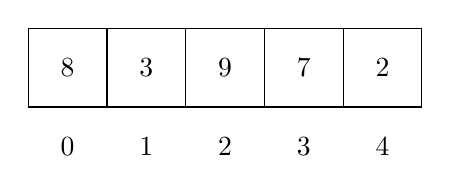
\begin{tikzpicture}
\draw (0,0) rectangle (1,1);
\draw (1,0) rectangle (2,1);
\draw (2,0) rectangle (3,1);
\draw (3,0) rectangle (4,1);
\draw (4,0) rectangle (5,1);

\node[scale=1] at (.5,0.5) {8};
\node[scale=1] at (1.5,0.5) {3};
\node[scale=1] at (2.5,0.5) {9};
\node[scale=1] at (3.5,0.5) {7};
\node[scale=1] at (4.5,0.5) {2};

\node[scale=1] at (0.5,-0.5) {0};
\node[scale=1] at (1.5,-0.5) {1};
\node[scale=1] at (2.5,-0.5) {2};
\node[scale=1] at (3.5,-0.5) {3};
\node[scale=1] at (4.5,-0.5) {4};
\end{tikzpicture}
\end{center}




\begin{center}
  \bgroup
  \def\arraystretch{1.5}%
  \begin{tabular}{ H  G  }
	\begin{lstlisting}[language=C++, caption=]
	sum(A,n) {
		s = 0;
		for( i=0 ; i<n ; i++ ) {
			s += A[i];
		}
		return s;
	}
	\end{lstlisting}
     &  
	\begin{lstlisting}[language=C++, caption=]
	.
	1
	n+1
	n
	.
	1
	.
	\end{lstlisting}
  \end{tabular}
  \egroup
\end{center}


Time Complexity :

\begin{align*}
\Rightarrow f(n) = 2n + 3 \Rightarrow O(n)
\end{align*}



Space Complexity :


\begin{align*}
\begin{rcases}
A &\to n \quad \\
n &\to 1 \\
s &\to 1 \\
i &\to 1 
\end{rcases}
\Rightarrow s(n) = n + 3 \Rightarrow O(n)
\end{align*}







\subsubsection{example}




\begin{center}
  \bgroup
  \def\arraystretch{1.5}%
  \begin{tabular}{ E  D  }
	\begin{lstlisting}[language=C++, caption=]
	add(A,B,n) {
		for( i=0 ; i<n ; i++ ) {
			for( j=0 ; j<n ; j++ ) {
				C[i,j] = A[i,j] + B[i,j];
			}
		}
	}
	\end{lstlisting}
     &  
	\begin{lstlisting}[language=C++, caption=]
	.
	n+1
	n * (n+1)
	n * n
	.
	.
	.
	\end{lstlisting}
  \end{tabular}
  \egroup
\end{center}


Time Complexity :


\begin{align*}
\Rightarrow f(n) = 2n^{2} + 2n + 1 \Rightarrow O(n^{2})
\end{align*}





Space Complexity :


\begin{align*}
\begin{rcases}
A &\to n^{2} \quad \\
B &\to n^{2} \\
C &\to n^{2} \\
n &\to 1 \\
i &\to 1 \\
j &\to 1 
\end{rcases}
\Rightarrow s(n) = 3n^{2} + 3 \Rightarrow O(n^{2})
\end{align*}






\subsubsection{example}




\begin{center}
  \bgroup
  \def\arraystretch{1.5}%
  \begin{tabular}{ E  C  }
	\begin{lstlisting}[language=C++, caption=]
	multiply(A,B,n) {
		for( i=0 ; i<n ; i++ ) {
			for( j=0 ; j<n ; j++ ) {
				C[i,j] = 0;
				for( k=0 ; k<n ; k++ ) {
					C[i,j] += A[i,k] * B[k,j];
				}
			}
		}
	}
	\end{lstlisting}
     &  
	\begin{lstlisting}[language=C++, caption=]
	.
	n+1
	n * (n+1)
	n * n
	n * n * (n+1)
	n * n * n
	.
	.
	.
	.
	\end{lstlisting}
  \end{tabular}
  \egroup
\end{center}


Time Complexity :


\begin{align*}
\Rightarrow f(n) = 2n^{3} + 3n^{2} + 2n + 1 \Rightarrow O(n^{3})
\end{align*}



Space Complexity :

\begin{align*}
\begin{rcases}
A &\to n^{2} \quad \\
B &\to n^{2} \\
C &\to n^{2} \\
n &\to 1 \\
i &\to 1 \\
j &\to 1 \\
k &\to 1 
\end{rcases}
\Rightarrow s(n) = 3n^{2} + 4 \Rightarrow O(n^{2})
\end{align*}





\section{Time Complexity 1th}


\subsubsection{example}


\begin{center}
  \bgroup
  \def\arraystretch{1.5}%
  \begin{tabular}{ H  G  }
	\begin{lstlisting}[language=C++, caption=]
	for( i=0 ; i<n ; i++ ) {
		statement;
	}
	\end{lstlisting}
     &  
	\begin{lstlisting}[language=C++, caption=]
	n+1
	n
	.
	\end{lstlisting}
  \end{tabular}
  \egroup
\end{center}




Time Complexity : $O(n)$





\subsubsection{example}


\begin{center}
  \bgroup
  \def\arraystretch{1.5}%
  \begin{tabular}{ H  G  }
	\begin{lstlisting}[language=C++, caption=]
	for( i=n ; i>0 ; i-- ) {
		statement;
	}
	\end{lstlisting}
     &  
	\begin{lstlisting}[language=C++, caption=]
	n+1
	n
	.
	\end{lstlisting}
  \end{tabular}
  \egroup
\end{center}




Time Complexity : $O(n)$



\subsubsection{example}


\begin{center}
  \bgroup
  \def\arraystretch{1.5}%
  \begin{tabular}{ H  C  }
	\begin{lstlisting}[language=C++, caption=]
	for( i=0 ; i<n ; i+=2 ) {
		statement;
	}
	\end{lstlisting}
     &  
	\begin{lstlisting}[language=C++, caption=]
	(n+1)/2
	n/2
	.
	\end{lstlisting}
  \end{tabular}
  \egroup
\end{center}




Time Complexity : $O(n)$



\subsubsection{example}


\begin{center}
  \bgroup
  \def\arraystretch{1.5}%
  \begin{tabular}{ H  C  }
	\begin{lstlisting}[language=C++, caption=]
	for( i=0 ; i<n ; i+=20 ) {
		statement;
	}
	\end{lstlisting}
     &  
	\begin{lstlisting}[language=C++, caption=]
	(n+1)/20
	n/20
	.
	\end{lstlisting}
  \end{tabular}
  \egroup
\end{center}




Time Complexity : $O(n)$



\subsubsection{example}



\begin{center}
  \bgroup
  \def\arraystretch{1.5}%
  \begin{tabular}{ E  D  }
	\begin{lstlisting}[language=C++, caption=]
	for( i=0 ; i<n ; i++ ) {
		for( j=0 ; j<n ; j++ ) {
			statement ;
		}
	}
	\end{lstlisting}
     &  
	\begin{lstlisting}[language=C++, caption=]
	n+1
	n * (n+1)
	n * n
	.
	.
	\end{lstlisting}
  \end{tabular}
  \egroup
\end{center}


Time Complexity : $O(n^{2})$






\subsubsection{example}



\begin{center}
  \bgroup
  \def\arraystretch{1.5}%
  \begin{tabular}{ E  D  }
	\begin{lstlisting}[language=C++, caption=]
	for( i=0 ; i<n ; i++ ) {
		for( j=0 ; j<i ; j++ ) {
			statement ;
		}
	}
	\end{lstlisting}
     &  
	\begin{lstlisting}[language=C++, caption=]
	n+1
	n * (n+1)
	n * n
	.
	.
	\end{lstlisting}
  \end{tabular}
  \egroup
\end{center}


Time Complexity : 


\begin{align*}
\Rightarrow 1 + 2 + 3 + \dots + n = \cfrac{n(n+1)}{2} \Rightarrow O(n^{2})
\end{align*}





\subsubsection{example}


\begin{center}
  \bgroup
  \def\arraystretch{1.5}%
  \begin{tabular}{ H  G  }
	\begin{lstlisting}[language=C++, caption=]
	for( i=0 ; i<n ; i*=2 ) {
		statement;
	}
	\end{lstlisting}
     &  
	\begin{lstlisting}[language=C++, caption=]

	\end{lstlisting}
  \end{tabular}
  \egroup
\end{center}



\begin{center}
  \bgroup
  \def\arraystretch{1.5}%
  \begin{tabular}{ l  }
	i
     \\ \hline
     $1$
     \\
     $1 \times 2 = 2$
     \\
     $2 \times 2 = 2^{2}$
     \\
     $2^{2} \times 2 = 2^{3}$
     \\
     $\vdots$
     \\
     $2^{k}$
     \\
  \end{tabular}
  \egroup
\end{center}




\begin{align*}
\Large
&2^{k}< n \\
\Rightarrow &\log^{2^{k}}_{2} < \log^{n}_{2}
\end{align*}


$\Rightarrow$ Time Complexity : $O(\log^{n}_{2})$

\vspace{30pt}

if n = 8 :


\begin{center}
  \bgroup
  \def\arraystretch{1.5}%
  \begin{tabular}{ l  }
	i
     \\ \hline
     $1 \to 2 \to 4 \to 8$
  \end{tabular}
  \egroup
\end{center}


$$
\ceil[\Big]{\log^{8}_{2}} = 3
$$




if n = 10 :


\begin{center}
  \bgroup
  \def\arraystretch{1.5}%
  \begin{tabular}{ l  }
	i
     \\ \hline
	$1 \to 2 \to 4 \to 8 \to 16$
  \end{tabular}
  \egroup
\end{center}


$$
\ceil[\Big]{\log^{10}_{2}} = \ceil[\Big]{3.2} = 4
$$





\subsubsection{example}

\begin{center}
  \bgroup
  \def\arraystretch{1.5}%
  \begin{tabular}{ H  G  }
	\begin{lstlisting}[language=C++, caption=]
	for( i=0 ; i<n ; i/=2 ) {
		statement;
	}
	\end{lstlisting}
     &  
	\begin{lstlisting}[language=C++, caption=]

	\end{lstlisting}
  \end{tabular}
  \egroup
\end{center}



\begin{center}
  \bgroup
  \def\arraystretch{1.5}%
  \begin{tabular}{ l  }
	i = n
     \\ \hline
     $\cfrac{n}{2} \to \cfrac{n}{2^{2}} \to \cfrac{n}{2^{3}} \to \cfrac{n}{2^{4}} \to \dots \to \cfrac{n}{2^{n}}$
  \end{tabular}
  \egroup
\end{center}


\begin{align*}
\Large
&\cfrac{n}{2^{k}} < 1 \\
\Rightarrow \quad & n < 2^{k} \\
\Rightarrow \quad & \log^{n}_{2} < \log^{2^{k}}_{2} \\
\Rightarrow \quad & \log^{n}_{2} < k \\
\Rightarrow \quad & k > \log^{n}_{2} \\
\end{align*}


$\Rightarrow$ Time Complexity : $O(\log^{n}_{2})$

%\vspace{30pt}



\newpage


\subsubsection{example}


\begin{center}
  \bgroup
  \def\arraystretch{1.5}%
  \begin{tabular}{ H  G  }
	\begin{lstlisting}[language=C++, caption=]
	for( i=0 ; i*i<n ; i++ ) {
		statement;
	}
	\end{lstlisting}
     &  
	\begin{lstlisting}[language=C++, caption=]

	\end{lstlisting}
  \end{tabular}
  \egroup
\end{center}


\begin{align*}
\Large
& i \times i \geq n  \\
& i^{2} \geq n  \\
& i \geq \sqrt{n}  \\
\end{align*}


$\Rightarrow$ Time Complexity : $O(\sqrt{n})$






\subsubsection{example}


\begin{center}
  \bgroup
  \def\arraystretch{1.5}%
  \begin{tabular}{ H  G  }
	\begin{lstlisting}[language=C++, caption=]
	for( i=0 ; i<n ; i++ ) {
		statement;
	}
	
	for( j=0 ; j<n ; j++ ) {
		statement;
	}
	\end{lstlisting}
     &  
	\begin{lstlisting}[language=C++, caption=]
	n+1
	n
	.
	.
	n+1
	n
	.
	\end{lstlisting}
  \end{tabular}
  \egroup
\end{center}


$\Rightarrow$ Time Complexity : $O(n)$







\subsubsection{example}


\begin{center}
  \bgroup
  \def\arraystretch{1.5}%
  \begin{tabular}{ H  C  }
	\begin{lstlisting}[language=C++, caption=]
	p = 0;
	for( i=0 ; i<n ; i*=2 ) {
		p += 1;
	}
	
	for( j=0 ; j<p ; j*=2 ) {
		statement;
	}
	\end{lstlisting}
     &  
	\begin{lstlisting}[language=C++, caption=]
	.
	.
	p = log(n)
	.
	.
	.
	log(p)
	.
	\end{lstlisting}
  \end{tabular}
  \egroup
\end{center}


$\Rightarrow$ Time Complexity : $O(\log{(\log{(n)})})$



\subsubsection{example}


\begin{center}
  \bgroup
  \def\arraystretch{1.5}%
  \begin{tabular}{ E  C  }
	\begin{lstlisting}[language=C++, caption=]
	for( i=0 ; i<n ; i++ ) {
		for( j=0 ; j<n ; j*=2) {
			statement ;
		}
	}
	\end{lstlisting}
     &  
	\begin{lstlisting}[language=C++, caption=]
	n
	n * log(n)
	n * log(n)
	.
	.
	\end{lstlisting}
  \end{tabular}
  \egroup
\end{center}



$\Rightarrow$ Time Complexity : $O(n \log{(n)})$





\section{Summary}



\begin{center}
  \bgroup
  \def\arraystretch{1.5}%
  \begin{tabular}{ E  C  }
	\begin{lstlisting}[language=C++, caption=]
	
	for( i=0 ; i<n ; i++ ) 
	\end{lstlisting}
     &
     { \Large  
	$O(n)$
	}
	\\ \hline
	\begin{lstlisting}[language=C++, caption=]
	
	for( i=0 ; i<n ; i+=2 ) 
	\end{lstlisting}
     &  
     { \Large  
	$O(n)$
	}
	\\ \hline
	\begin{lstlisting}[language=C++, caption=]
	
	for( i=n ; i>1 ; i-- ) 
	\end{lstlisting}
     &  
     { \Large  
	$O(n)$
	}
	\\ \hline
	\begin{lstlisting}[language=C++, caption=]
	
	for( i=1 ; i<n ; i*=2 ) 
	\end{lstlisting}
     &  
     { \Large  
	$O(\log^{n}_{2})$
	}
	\\ \hline
	\begin{lstlisting}[language=C++, caption=]
	
	for( i=0 ; i<n ; i*=3 ) 
	\end{lstlisting}
     &  
     { \Large  
	$O(\log^{n}_{3})$
	}
	\\ \hline
	\begin{lstlisting}[language=C++, caption=]
	
	for( i=n ; i>1 ; i/=2 ) 
	\end{lstlisting}
     &  
     { \Large  
	$O(\log^{n}_{2})$
	}
	\\ 
  \end{tabular}
  \egroup
\end{center}





\section{Analysis of while loop}


\subsubsection{example}

\begin{center}
  \bgroup
  \def\arraystretch{1.5}%
  \begin{tabular}{ H  G  }
	\begin{lstlisting}[language=C++, caption=]
	for( i=0 ; i*i<n ; i++ ) {
		statement;
	}
	\end{lstlisting}
     &  
	\begin{lstlisting}[language=C++, caption=]
	n+1 
	n
	.
	\end{lstlisting}
  \end{tabular}
  \egroup
\end{center}



$f(n) = 2n + 1 \Rightarrow$ Time Complexity : $O(n)$


\begin{center}
  \bgroup
  \def\arraystretch{1.5}%
  \begin{tabular}{ H  G  }
	\begin{lstlisting}[language=C++, caption=]
	i = 0;
	while(i < n) {
		statement;
		i++;
	}
	\end{lstlisting}
     &  
	\begin{lstlisting}[language=C++, caption=]
	1
	n+1
	n
	n
	.
	\end{lstlisting}
  \end{tabular}
  \egroup
\end{center}


$f(n) = 3n + 2 \Rightarrow$ Time Complexity : $O(n)$





\subsubsection{example}



\begin{center}
  \bgroup
  \def\arraystretch{1.5}%
  \begin{tabular}{ H  G  }
	\begin{lstlisting}[language=C++, caption=]
	i = 0;
	while(i < n) {
		statement;
		i*=2;
	}
	\end{lstlisting}
  \end{tabular}
  \egroup
\end{center}




\begin{center}
  \bgroup
  \def\arraystretch{1.5}%
  \begin{tabular}{ l  }
	i
     \\ \hline
     $1$
     \\
     $1 \times 2 = 2$
     \\
     $2 \times 2 = 2^{2}$
     \\
     $2^{2} \times 2 = 2^{3}$
     \\
     $\vdots$
     \\
     $2^{k}$
     \\
  \end{tabular}
  \egroup
\end{center}




\begin{align*}
\Large
&2^{k}< n \\
\Rightarrow \quad &\log^{2^{k}}_{2} < \log^{n}_{2} \\
\Rightarrow \quad &k < \log^{n}_{2} 
\end{align*}


$\Rightarrow$ Time Complexity : $O(\log^{n}_{2})$




\subsubsection{example}






\begin{center}
  \bgroup
  \def\arraystretch{1.5}%
  \begin{tabular}{ H  G  }
	\begin{lstlisting}[language=C++, caption=]
	i = 1;
	k = 1;
	while(k < n) {
		statement;
		k+=i;
		i++;
	}
	\end{lstlisting}
  \end{tabular}
  \egroup
\end{center}





\begin{center}
  \bgroup
  \def\arraystretch{1.5}%
  \begin{tabular}{ l  l }
	i & k
     \\ \hline
     1 & 1
     \\
     2 & 1+1 
     \\
     3 & 1 + 1 + 2 
     \\
     4 & 1 + 1 + 2 + 3
     \\
     $\vdots$ & $\vdots$
     \\
     m & 1 + 1 + 2 + 3 + \dots + m = $\cfrac{m(m+1)}{2}$
     \\
  \end{tabular}
  \egroup
\end{center}


\begin{align*}
\Large
&k < n \\
\Rightarrow \quad & \cfrac{m(m+1)}{2} < n \\
\Rightarrow \quad & m^{2} < n \\
\Rightarrow \quad & m < \sqrt{n} \\
\end{align*}


$\Rightarrow$ Time Complexity : $O(\sqrt{n})$







\section{Analysis of if statement}


\begin{center}
  \bgroup
  \def\arraystretch{1.5}%
  \begin{tabular}{ H  G  }
	\begin{lstlisting}[language=C++, caption=]
	Test(n) {
		if(n < 5) {
			print(n);
		} else {
			for(i=0;i<n;i++) {
				print(n);
			}
		}
	}
	\end{lstlisting}
	&
	\begin{lstlisting}[language=C++, caption=]
	.
	.
	1
	.
	n+1
	n
	.
	.
	.
	\end{lstlisting}
  \end{tabular}
  \egroup
\end{center}


\begin{align*}
\text{Time Complexity} \Rightarrow
\begin{cases}
Worst &\to O(1) \\
Best &\to O(n) \\
\end{cases}
\end{align*}



\section{Classes of Functions}




\begin{center}
  \bgroup
  \def\arraystretch{1.5}%
  \begin{tabular}{ l | l  }
	$O(1)$
	&
	constant
	\\ \hline
	$O(\log{n})$
	&
	Logarithmic
	\\ \hline
	$O(n)$
	&
	Linear
	\\ \hline
	$O(n^{2})$
	&
	Quadratic
	\\ \hline
	$O(n^{3})$
	&
	Cubic
	\\ \hline
	$O(2^{n})$
	&
	Exponential
	\\ \hline
	$O(3^{n})$
	&
	
	\\ \hline
	$O(n!)$
	&
	
	\\ \hline
	$O(n^{n})$
	&
	
	\\ 
  \end{tabular}
  \egroup
\end{center}






\section{Compare Classes of Functions}




\begin{align*}
1 < \log{n} < \sqrt{n} < n < n\log{n} < n^{2} < n^{3} < 2^{n} < 3^{n} < n! < n^{n}
\end{align*}






\section{Asymptotic Notation}




\begin{center}
  \bgroup
  \def\arraystretch{1.5}%
  \begin{tabular}{ l | l | l }
	$O$ 
	&
	big-oh
	&
	Upper Bound
	\\ \hline
	$\Omega$ 
	&
	big-Omega
	&
	Lower Bound
	\\ \hline
	$\theta$ 
	&
	theta
	&
	Average Bound
	\\ 
  \end{tabular}
  \egroup
\end{center}




\subsection{Big oh - $O$}

\begin{tcolorbox}
the function
$f(n) = O(g(n))$
if there exists 
c and $n_{0}$
such that 

$$
f(n) \leq c \times g(n) \quad \forall \quad n \geq n_{0}
$$
\end{tcolorbox}


\subsubsection{example}


$f(n) = 2n + 3$

if $c = 10$ :

\begin{align*}
\underbrace{2n+3}_{f(n)} \leq \underbrace{10}_{c} \times \underbrace{n}_{g(n)} 
\end{align*}

$$
\Rightarrow f(n) = O(n)
$$


\subsection{Big omega - $\Omega$}


\begin{tcolorbox}
the function
$f(n) = \Omega(g(n))$
if there exists 
c and $n_{0}$
such that 

$$
f(n) \geq c \times g(n) \quad \forall \quad n \geq n_{0}
$$
\end{tcolorbox}




\subsubsection{example}


$f(n) = 2n + 3$

if $c = 1$ :

\begin{align*}
\underbrace{2n+3}_{f(n)} \geq \underbrace{1}_{c} \times \underbrace{n}_{g(n)} 
\end{align*}

$$
\Rightarrow f(n) = \Omega(n)
$$





\subsection{theta - $\theta$}


\begin{tcolorbox}
the function
$f(n) = \theta(g(n))$
if there exists 
$c_{1}$ , $c_{2}$ and $n_{0}$
such that 

$$
c_{1} \times g(n) \leq f(n) \leq c_{2} \times g(n) \quad \forall \quad n \geq n_{0}
$$
\end{tcolorbox}



\subsubsection{example}


$f(n) = 2n + 3$

if $c_{1} = 1$ and  $c_{2} = 10$:

\begin{align*}
\underbrace{1}_{c_{1}} \times \underbrace{n}_{g(n)}  \leq  \underbrace{2n+3}_{f(n)} \leq \underbrace{10}_{c_{2}} \times \underbrace{n}_{g(n)} 
\end{align*}

$$
\Rightarrow f(n) = \theta(n)
$$



\section{Asymptotic Notation - examples}







\subsubsection{example}


$f(n) = 2n^{2} + 3n + 4$

if $c = 9$ and $g(n) = n^{2}$ :

\begin{align*}
\underbrace{2n^{2} + 3n + 4}_{f(n)} \leq \underbrace{9}_{c} \times \underbrace{n^{2}}_{g(n)} 
\end{align*}

$$
\Rightarrow f(n) = O(n^{2})
$$



if $c = 1$ and $g(n) = n^{2}$ :

\begin{align*}
\underbrace{2n^{2} + 3n + 4}_{f(n)} \geq \underbrace{1}_{c} \times \underbrace{n^{2}}_{g(n)} 
\end{align*}

$$
\Rightarrow f(n) = \Omega(n^{2})
$$


if $c_{1} = 1$ and  $c_{2} = 9$ and $g(n) = n^{2}$ :

\begin{align*}
\underbrace{1}_{c_{1}} \times \underbrace{n^{2}}_{g(n)}  \leq  \underbrace{2n^{2} + 3n + 4}_{f(n)} \leq \underbrace{9}_{c_{2}} \times \underbrace{n^{2}}_{g(n)} 
\end{align*}

$$
\Rightarrow f(n) = \theta(n^{2})
$$











\subsubsection{example}


$f(n) = n^{2}\log{n} + n$

if $c = 10$ and $g(n) = n^{2}\log{n}$ :

\begin{align*}
\underbrace{n^{2}\log{n} + n}_{f(n)} \leq \underbrace{10}_{c} \times \underbrace{n^{2}\log{n}}_{g(n)} 
\end{align*}

$$
\Rightarrow f(n) = O(n^{2}\log{n})
$$



if $c = 1$ and $g(n) = n^{2}\log{n}$ :

\begin{align*}
\underbrace{n^{2}\log{n} + n}_{f(n)} \geq \underbrace{1}_{c} \times \underbrace{n^{2}\log{n}}_{g(n)} 
\end{align*}

$$
\Rightarrow f(n) = \Omega(n^{2}\log{n})
$$


if $c_{1} = 1$ and  $c_{2} = 10$:

\begin{align*}
\underbrace{1}_{c_{1}} \times \underbrace{n^{2}\log{n}}_{g(n)}  \leq  \underbrace{n^{2}\log{n} + n}_{f(n)} \leq \underbrace{10}_{c_{2}} \times \underbrace{n^{2}\log{n}}_{g(n)} 
\end{align*}

$$
\Rightarrow f(n) = \theta(n^{2}\log{n})
$$





\subsubsection{example}


$$
f(n) = n!
$$

$$
n! = 1 \times 2 \times 3 \times \dots \times (n-1) \times n
$$


$$
1 \times 1 \times 1 \times \dots \times 1 
\leq 
1 \times 2 \times 3 \times \dots \times (n-1) \times n 
\leq
n \times n \times n \times \dots \times n 
$$


$$
1 \leq n! \leq n^{n}
$$



$$
\Rightarrow \begin{cases}
O(n^{n}) 
\\
\Omega(1)
\end{cases}
$$





\subsubsection{example}



$$
f(n) = \log{(n!)}
$$


$$
\log{(1 \times 1 \times 1 \times \dots \times 1)}
\leq 
\log{(1 \times 2 \times 3 \times \dots \times (n-1) \times n) }
\leq
\log{(n \times n \times n \times \dots \times n) }
$$



$$
1 \leq \log{(n!)} \leq \log{(n^{n})} \Rightarrow 1 \leq \log{(n!)} \leq n\log{(n)}
$$



$$
\Rightarrow \begin{cases}
O(n\log{(n)}) 
\\
\Omega(1)
\end{cases}
$$


\newpage


\section{Properties of Asymptotic Notations}



\subsection{General Properties}

\begin{tcolorbox}
if 
$f(n)$
 is 
$O(g(n))$
then
$a \times f(n)$
 is 
$O(g(n))$
\end{tcolorbox}

e.g : 

$f(n) = 2n^{2} + 5$
is
$O(n^{2})$

then 
$7 \times f(n) = 7 \times (2n^{2} + 5)$
is
$O(n^{2})$


\begin{tcolorbox}
if 
$f(n)$
 is 
$\Omega(g(n))$
then
$a \times f(n)$
 is 
$\Omega(g(n))$
\end{tcolorbox}


e.g : 

$f(n) = 2n^{2} + 5$
is
$\Omega(n^{2})$

then 
$7 \times f(n) = 7 \times (2n^{2} + 5)$
is
$\Omega(n^{2})$

\subsection{Reflexive}

\begin{tcolorbox}
if
$f(n)$
is given 
then we have
$O(f(n))$
\end{tcolorbox}

e.g : 

$f(n) = n^{2} \Rightarrow f(n) = O(n^{2})$



\subsection{Transitive}

\begin{tcolorbox}
if
$f(n)$
is 
$O(g(n))$
and
$g(n)$
is 
$O(h(n))$
then
$f(n) = O(h(n))$
\end{tcolorbox}


e.g : $f(n) = n \quad g(n) = n^{2} \quad h(n) = n^{3}$


\begin{align*}
\begin{rcases}
n \to O(n^{2}) \\
n^{2} \to  O(n^{3}) \\
\end{rcases}
\Rightarrow f(n) = O(n^{3})
\end{align*}




\subsection{Transitive}

\begin{tcolorbox}
if
$f(n)$
is 
$\theta(g(n))$
then
$g(n)$
is 
$\theta(f(n))$
\end{tcolorbox}



e.g : 

$f(n) = n^{2} \quad g(n) = n^{2}$

$f(n) = \theta(n^{2})$

$g(n) = \theta(n^{2})$





\subsection{Transpose Symmetric}

\begin{tcolorbox}
if
$f(n)$
is 
$O(g(n))$
then
$g(n)$
is 
$\Omega(f(n))$
\end{tcolorbox}


e.g : 


$f(n) = n \quad  \Rightarrow \quad f(n) = O(n^{2})$

$g(n) = n^{2} \quad \Rightarrow \quad g(n) = \Omega(n)$






\subsection{point}

\begin{tcolorbox}
if
$f(n) = O(g(n))$
and
$f(n) = \Omega(g(n))$
then we have :
\end{tcolorbox}


$$
g(n) \leq  f(n)  \leq g(n) \quad \Rightarrow \quad f(n) = \theta(g(n))
$$




\subsection{point}

\begin{tcolorbox}
if
$f(n) = O(g(n))$
and
$d(n) = O(e(n))$
then we have :
$$
f(n) + d(n) = O( max(g(n),e(n)) )
$$
\end{tcolorbox}


e.g : 

$f(n) = n^{2} \to O(n^{2})$

$d(n) = n \to O(n)$

$$
f(n) + d(n) = n^{2} + n =  O( n^{2} )
$$





\subsection{point}

\begin{tcolorbox}
if
$f(n) = O(g(n))$
and
$d(n) = O(e(n))$
then we have :
$$
f(n) \times d(n) = O( g(n) \times e(n) )
$$
\end{tcolorbox}


e.g : 

$f(n) = n^{2} \to O(n^{2})$

$d(n) = n \to O(n)$

$$
f(n) \times d(n) = n^{2} \times n = n^{3} =  O( n^{3} )
$$


\newpage

\section{Comparision of functions}

{
\LARGE
\begin{align*}
f(n) = 3 n^{\sqrt{n}}  \qquad g(n) = 2^{\sqrt{n}\log^{n}_{2}} 
\end{align*}
}

\begin{tcolorbox}
\LARGE
\begin{align*}
a^{\log^{b}_{c}} = b^{\log^{a}_{c}}
\end{align*}
\end{tcolorbox}


{
\LARGE
\begin{align*}
g(n) &= 2^{\sqrt{n}\log^{n}_{2}} \\
&= 2^{\log^{n^{\sqrt{n}}}_{2}} \\
&= (n^{\sqrt{n}})^{\log^{2}_{2}} \\
&= n^{\sqrt{n}} \\
\\
\Rightarrow \quad &3 n^{\sqrt{n}} > n^{\sqrt{n}} 
\end{align*}
}



\newpage

\section{Recurrence Relation}


\subsubsection{example}


\begin{center}
  \bgroup
  \def\arraystretch{1.5}%
  \begin{tabular}{ E  D  }
	\begin{lstlisting}[language=C++, caption=]
	Test(n) {
		if(n > 0) {
			print(n);
			Test(n-1);
		}
	}
	\end{lstlisting}
     &  
	\begin{lstlisting}[language=C++, caption=]
	T(n)
	.
	1
	T(n-1)
	.
	.
	\end{lstlisting}
  \end{tabular}
  \egroup
\end{center}



$$
T(n) = T(n-1) + 1
$$



$$
T(n) = \begin{cases}
1  &n = 0 \\
T(n-1) + 1  &n > 0 \\
\end{cases}
$$





\begin{center}
\begin{tikzpicture}[sibling distance = 2cm]
\node (root0) {T(n)}
child {node {1}}
child {node (root1) {T(n-1)}
	child {node {1}}
	child {node (root2) {T(n-2)}
		child {node {1}}
		child {node (root3) {T(n-3)}
			child {node {1}}
			child {node (root4) {$\vdots$}
				child {node (root5) {$T(0)$}}
			}
	} }
};

\node (one0) at ($(root0)+(6,0)$) {1};
\node (one1) at ($(root1)+(5,0)$) {1};
\node (one2) at ($(root2)+(4,0)$) {1};
\node (one3) at ($(root3)+(3,0)$) {1};
\node (one4) at ($(root4)+(2,0)$) {$\vdots$};
\node (one5) at ($(root5)+(2,0)$) {1};
%\node (one0) at (7,0) {1};
%\node (one1) at (7,-1) {1};
%\node (one2) at (7,-2) {1};
%\node (one3) at (7,-3) {1};

\draw[dashed] (root0) -- (one0);
\draw[dashed] (root1) -- (one1);
\draw[dashed] (root2) -- (one2);
\draw[dashed] (root3) -- (one3);
%\draw[dashed] (root4) -- (one4);
\draw[dashed] (root5) -- (one5);
\end{tikzpicture}
\end{center}




\begin{align*}
1 + 1 + 1 + \dots + 1 = n \Rightarrow f(n) = O(n)
\end{align*}



\begin{align*}
&T(n) = T(n-1) + 1 \\
&T(n-1) = T(n-2) + 1 \\
\text{substitute}& \\
\Rightarrow \quad &T(n) = [ T(n-2) + 1 ] + 1 \\
\Rightarrow \quad &T(n) =  T(n-2) + 2 \\
&T(n-2) = T(n-3) + 1 \\
\text{substitute} \\
\Rightarrow \quad &T(n) = [ T(n-3) + 1 ] + 2 \\
\Rightarrow \quad &T(n) =  T(n-3) + 3 \\
\text{continue for k times}& \\
\Rightarrow \quad &T(n) =  T(n-k) + k \\
\end{align*}



\begin{align*}
k = n \\
\Rightarrow \quad &T(n) = T(n-n) + n \\
\Rightarrow \quad &T(n) = T(0) + n \\
\Rightarrow \quad &T(n) = 1 + n \\
\begin{rcases}
&f(n) = O(n) \\
&f(n) = \Omega(n) 
\end{rcases}
\Rightarrow \quad &f(n) = \theta(n) 
\end{align*}




\subsubsection{example}




\begin{center}
  \bgroup
  \def\arraystretch{1.5}%
  \begin{tabular}{ E  D  }
	\begin{lstlisting}[language=C++, caption=]
	Test(n) {
		if(n > 0) {
			for(i=0;i<n;i++) {
				print(n);
			}
			Test(n-1);
		}
	}
	\end{lstlisting}
     &  
	\begin{lstlisting}[language=C++, caption=]
	T(n)
	.
	n+1
	n
	.
	T(n-1)
	.
	.
	\end{lstlisting}
  \end{tabular}
  \egroup
\end{center}



$$
T(n) = T(n-1) + n
$$



$$
T(n) = 
\begin{cases}
1  &n = 0 \\
T(n-1) + n  &n > 0 \\
\end{cases}
$$






\begin{center}
\begin{tikzpicture}[sibling distance = 2cm]
\node (root0) {T(n)}
child {node {n}}
child {node (root1) {T(n-1)}
	child {node {n-1}}
	child {node (root2) {T(n-2)}
		child {node {n-2}}
		child {node (root3) {T(n-3)}
			child {node {n-3}}
			child {node (root4) {$\vdots$}
				child {node (root5) {$T(0)$}}
			}
	} }
};

\node (one0) at ($(root0)+(6,0)$) {$n$};
\node (one1) at ($(root1)+(5,0)$) {$n-1$};
\node (one2) at ($(root2)+(4,0)$) {$n-2$};
\node (one3) at ($(root3)+(3,0)$) {$n-3$};
\node (one4) at ($(root4)+(2,0)$) {$\vdots$};
\node (one5) at ($(root5)+(2,0)$) {$1$};

%\node (one0) at (7,0) {1};
%\node (one1) at (7,-1) {1};
%\node (one2) at (7,-2) {1};
%\node (one3) at (7,-3) {1};

\draw[dashed] (root0) -- (one0);
\draw[dashed] (root1) -- (one1);
\draw[dashed] (root2) -- (one2);
\draw[dashed] (root3) -- (one3);
%\draw[dashed] (root4) -- (one4);
\draw[dashed] (root5) -- (one5);
\end{tikzpicture}
\end{center}




\begin{align*}
0 + 1 + 2 + \dots + (n-2) + (n-1) + n = \frac{n(n+1)}{2} \Rightarrow f(n) = O(n^{2})
\end{align*}






\begin{align*}
&T(n) = T(n-1) + n \\
&T(n-1) = T(n-2) + n-1 \\
\text{substitute}& \\
\Rightarrow \quad &T(n) = \left[ T(n-2) + n-1 \right] + n \\
\Rightarrow \quad &T(n) =  T(n-2) + n-1 + n  \\
&T(n-2) = T(n-3) + n-2 \\
\text{substitute} \\
\Rightarrow \quad &T(n) = [ T(n-3) + n-2 ] + n-1 + n \\
\Rightarrow \quad &T(n) =  T(n-3) + n-2 + n-1 + n \\
\text{continue for k times}& \\
\Rightarrow \quad &T(n) =  T(n-k) + (n-(k-1)) + \dots  + n-2 + n-1 + n \\
\end{align*}



\begin{align*}
k = n \\
\Rightarrow \quad &T(n) = T(n-n) + n-(n-1) + \dots  + n-2 + n-1 + n \\
\Rightarrow \quad &T(n) = T(0) + 1 + \dots  + n-2 + n-1 + n \\
\Rightarrow \quad &T(n) = T(0) + 1 + 2 + 3 + \dots  + n-2 + n-1 + n \\
\Rightarrow \quad &T(n) = 1 + \cfrac{n(n+1)}{2} \\
\begin{rcases}
&f(n) = O(n^{2}) \\
&f(n) = \Omega(n^{2}) 
\end{rcases}
\Rightarrow \quad &f(n) = \theta(n^{2}) 
\end{align*}






\subsubsection{example}





\begin{center}
  \bgroup
  \def\arraystretch{1.5}%
  \begin{tabular}{ E  D  }
	\begin{lstlisting}[language=C++, caption=]
	Test(n) {
		if(n > 0) {
			for(i=0;i<n;i*=2) {
				print(n);
			}
			Test(n-1);
		}
	}
	\end{lstlisting}
     &  
	\begin{lstlisting}[language=C++, caption=]
	T(n)
	.
	.
	log(n)
	.
	T(n-1)
	.
	.
	\end{lstlisting}
  \end{tabular}
  \egroup
\end{center}



$$
T(n) = T(n-1) + \log{(n)}
$$



$$
T(n) = 
\begin{cases}
1  &n = 0 \\
T(n-1) + \log{(n)}  &n > 0 \\
\end{cases}
$$







\begin{center}
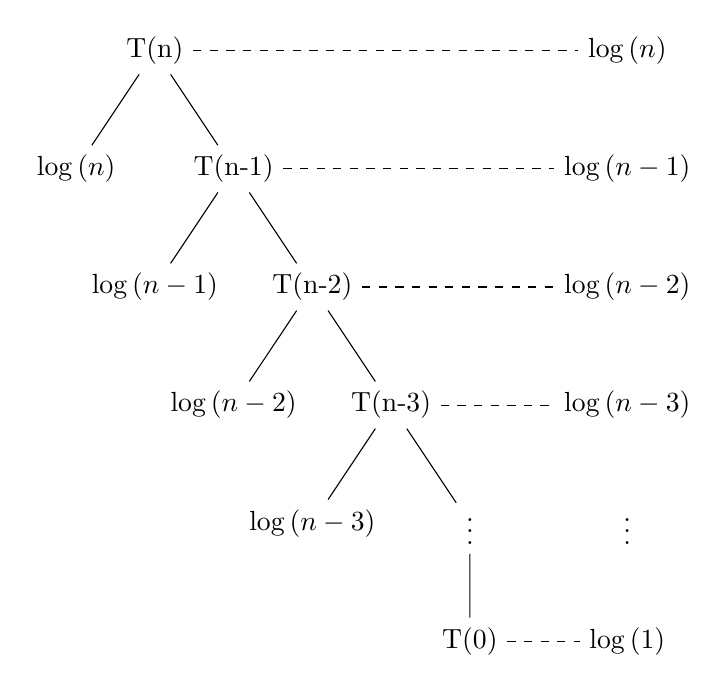
\begin{tikzpicture}[sibling distance = 2cm]
\node (root0) {T(n)}
child {node {$\log{(n)}$}}
child {node (root1) {T(n-1)}
	child {node {$\log{(n-1)}$}}
	child {node (root2) {T(n-2)}
		child {node {$\log{(n-2)}$}}
		child {node (root3) {T(n-3)}
			child {node {$\log{(n-3)}$}}
			child {node (root4) {$\vdots$}
				child {node (root5) {T(0)}}
			}
	} }
};


\node (one0) at ($(root0)+(6,0)$) {$\log{(n)}$};
\node (one1) at ($(root1)+(5,0)$) {$\log{(n-1)}$};
\node (one2) at ($(root2)+(4,0)$) {$\log{(n-2)}$};
\node (one3) at ($(root3)+(3,0)$) {$\log{(n-3)}$};
\node (one4) at ($(root4)+(2,0)$) {$\vdots$};
\node (one5) at ($(root5)+(2,0)$) {$\log{(1)}$};

%\node (one0) at (7,0) {1};
%\node (one1) at (7,-1) {1};
%\node (one2) at (7,-2) {1};
%\node (one3) at (7,-3) {1};

\draw[dashed] (root0) -- (one0);
\draw[dashed] (root1) -- (one1);
\draw[dashed] (root2) -- (one2);
\draw[dashed] (root3) -- (one3);
%\draw[dashed] (root4) -- (one4);
\draw[dashed] (root5) -- (one5);
\end{tikzpicture}
\end{center}




\begin{align*}
&\log{(n)} + \log{(n-1)} + \log{(n-2)} + \dots + \log{(2)} + \log{(1)} \\
&= \log{(n) \times (n-1) \times (n-2) \times \dots \times 2 \times 1} \\
&= \log{(n!)}\\
& \colorbox{gray!10}{\parbox{90pt}{
    $$n! < n^{n}$$
}}
\\
& \colorbox{gray!10}{\parbox{270pt}{
    $$\underbrace{n \times (n-1) \times \dots \times 2 \times 1}_{n!} < \underbrace{n \times n \times n \times \dots \times n}_{n^n}$$
}}
\\
& \colorbox{gray!10}{\parbox{180pt}{
    $$O(\log{(n!)}) < O(n\log{(n)})$$
}}
\\
&\Rightarrow f(n) = O(n\log{(n)})
\end{align*}









\begin{align*}
&T(n) = T(n-1) + \log{(n)} \\
&T(n-1) = T(n-2) + \log{(n-1)} \\
\text{substitute}& \\
\Rightarrow \quad &T(n) = \left[ T(n-2) + \log{(n-1)} \right] + \log{(n)} \\
\Rightarrow \quad &T(n) =  T(n-2) + \log{(n-1)} + \log{(n)}  \\
&T(n-2) = T(n-3) + \log{(n-2)} \\
\text{substitute} \\
\Rightarrow \quad &T(n) = [ T(n-3) + \log{(n-2)} ] + \log{(n-1)} + \log{(n)} \\
\Rightarrow \quad &T(n) =  T(n-3) + \log{(n-2)} + \log{(n-1)} + \log{(n)} \\
\text{continue for k times}& \\
\Rightarrow \quad &T(n) =  T(n-k) + \log{(n-(k-1))} + \dots + \log{(n-2)} + \log{(n-1)} + \log{(n)} \\
\Rightarrow \quad &T(n) =  T(n-k) + \log{(n-(k-1))} + \dots + \log{(n-2)} + \log{(n-1)} + \log{(n)} \\
\end{align*}



\begin{align*}
k = n \\
\Rightarrow \quad &T(n) =  T(n-n) + \log{(n-(n-1))} + \dots + \log{(n-2)} + \log{(n-1)} + \log{(n)} \\
\Rightarrow \quad &T(n) =  T(n-n) + \log{(1)} + \dots + \log{(n-2)} + \log{(n-1)} + \log{(n)} \\
\Rightarrow \quad &T(n) =  T(0) + \log{(1)} + \log{(2)} + \dots + \log{(n-2)} + \log{(n-1)} + \log{(n)} \\
\Rightarrow \quad &T(n) = 1 + \log{(n!)} \\
&\begin{rcases}
&f(n) = O(n\log{(n)}) \\
&f(n) = \Omega(n\log{(n)}) 
\end{rcases}
\Rightarrow \quad f(n) = \theta(n\log{(n)}) 
\end{align*}






\section{Summary}





\begin{center}
  \bgroup
  \def\arraystretch{1.5}%
  \begin{tabular}{ l | l  }
	$T(n) = T(n-1) + 1$
	&
	{ \Large  
	$O(n)$
	}
	\\ \hline
	$T(n) = T(n-1) + n$
	&
	{ \Large  
	$O(n^{2})$
	}
	\\ \hline
	$T(n) = T(n-1) + \log{(n)}$
	&
	{ \Large  
	$O(n\log{(n)})$
	}
	\\ \hline
	$T(n) = T(n-1) + n^{2}$
	&
	{ \Large  
	$O(n^{3})$
	}
	\\ \hline
	$T(n) = T(n-1) + 1$
	&
	{ \Large  
	$O(n)$
	}
	\\ \hline
	$T(n) = T(n-2) + 1$
	&
	{ \Large  
	$O(\frac{n}{2}) = O(n)$
	}
	\\ \hline
	$T(n) = T(n-100) + n$
	&
	{ \Large  
	$O(n^{2})$
	}
	\\ 
  \end{tabular}
  \egroup
\end{center}







\newpage



\subsubsection{example}





\begin{center}
  \bgroup
  \def\arraystretch{1.5}%
  \begin{tabular}{ E  D  }
	\begin{lstlisting}[language=C++, caption=]
	Test(n) {
		if(n > 0) {
			print(n);
			Test(n-1);
			Test(n-1);
		}
	}
	\end{lstlisting}
     &  
	\begin{lstlisting}[language=C++, caption=]
	T(n)
	.
	1
	T(n-1)
	T(n-1)
	.
	.
	\end{lstlisting}
  \end{tabular}
  \egroup
\end{center}



$$
T(n) = 2T(n-1) + 1
$$



$$
T(n) = 
\begin{cases}
1  &n = 0 \\
2T(n-1) + 1  &n > 0 \\
\end{cases}
$$









\begin{center}
\begin{tikzpicture}
\tikzstyle{level 1}=[sibling distance=6cm,level distance = 4cm]
\tikzstyle{level 2}=[sibling distance=2cm,level distance = 3cm]
\tikzstyle{level 3}=[sibling distance=0.6cm,level distance = 2cm]
\node (root0) {T(n)}
child {node {1}}
child {node (root11) {T(n-1)}
	child {node {1}}
	child {node (root21) {T(n-2)}
		child {node {1}}
		child {  [fill] circle (2pt)
			child {node {$\vdots$}}
		}
		child {  [fill] circle (2pt)
			child {node {$\vdots$}}
		}
	}
	child {node (root22) {T(n-2)}
		child {node {1}}
		child {  [fill] circle (2pt)
			child {node {$\vdots$}}
		}
		child { [fill] circle (2pt)
			child {node {$\vdots$}}
		}
	}
}
child {node (root12) {T(n-1)}
	child {node {1}}
	child {node (root23) {T(n-2)}
		child {node {1}}
		child { [fill] circle (2pt)
			child {node {$\vdots$}}
		}
		child {  [fill] circle (2pt)
			child {node {$\vdots$}}
		}
	}
	child {node (root24) {T(n-2)}
		child {node {1}}
		child {  [fill] circle (2pt)
			child {node {$$}}
		}
		child { [fill] circle (2pt) node (root38) {} 
			child {node (root416) {T(n-k)}}
		}
	}
};
\node (one0) at ($(root0)+(10.5,0)$) {$1 = 2^{0}$};
\node (one1) at ($(root12)+(4.5,0)$) {$2 = 2^{1}$};
\node (one2) at ($(root24)+(2.5,0)$) {$4 = 2^{2}$};
\node (one3) at ($(root38)+(2,0)$) {$8 = 2^{3}$};
\node (one4) at ($(root416)+(2,0)$) {$2^{k}$};

%\node (one0) at (7,0) {1};
%\node (one1) at (7,-1) {1};
%\node (one2) at (7,-2) {1};
%\node (one3) at (7,-3) {1};

\draw[dashed] (root0) -- (one0);
\draw[dashed] (root12) -- (one1);
\draw[dashed] (root24) -- (one2);
\draw[dashed] (root38) -- (one3);
\draw[dashed] (root416) -- (one4);
\end{tikzpicture}
\end{center}





\begin{tcolorbox}
$$a + ar + ar^{2} + ar^{3} + \dots + ar^{k} = \cfrac{a(r^{k+1} - 1)}{r-1}$$
\end{tcolorbox}



\begin{align*}
\begin{rcases}
&a = 1
\\
&r = 2
\end{rcases} \Rightarrow
1 + 2 + 2^{2} + 2^{3} + \dots + 2^{k} = \cfrac{1 \times  (2^{k+1} - 1)}{2-1} = 2^{k+1} - 1
\end{align*}




\begin{align*}
&n = k \\
\Rightarrow &f(n) = 2^{n+1} - 1 \\
\Rightarrow &f(n) = O(2^{n})
\end{align*}







\begin{align*}
&T(n) = 2 T(n-1) + 1 \\
&T(n-1) = 2 T(n-2) + 1 \\
\text{substitute}& \\
\Rightarrow \quad &T(n) = 2 [ 2T(n-2) + 1 ] + 1 \\
\Rightarrow \quad &T(n) =  2^{2} T(n-2) + 2 + 1\\
&T(n-2) = 2T(n-3) + 1 \\
\text{substitute} \\
\Rightarrow \quad &T(n) = 2^{2}[ 2T(n-3) + 1 ] + 2 + 1 \\
\Rightarrow \quad &T(n) =  2^{3}T(n-3) + 2^{2} + 2 +1 \\
\text{continue for k times}& \\
\Rightarrow \quad &T(n) =  2^{k}T(n-k) + 2^{k-1} + \dots + 2^{3} + 2^{2} + 2 + 1 \\
\end{align*}







\begin{align*}
\Rightarrow \quad &T(n) = 2^{k}T(n-k) + 2^{k-1} + \dots + 2^{3} + 2^{2} + 2 + 1 \\
k = n \\
\Rightarrow \quad &T(n) = 2^{n}T(n-n) + 2^{n-1} + \dots + 2^{3} + 2^{2} + 2 + 1 \\
\Rightarrow \quad &T(n) = 2^{n}T(n-n) + 2^{n-1} + \dots + 2^{3} + 2^{2} + 2 + 1 \\
\Rightarrow \quad &T(n) = 2^{n}\underbrace{T(0)}_{1} + 2^{n} - 1 \\
\Rightarrow \quad &T(n) = 2^{n}+ 2^{n} - 1 \\
\Rightarrow \quad &T(n) = 2 \times  2^{n} - 1 \\
\Rightarrow \quad &T(n) = 2^{n+1} - 1 \\
\begin{rcases}
&f(n) = O(2^{n}) \\
&f(n) = \Omega(2^{n}) 
\end{rcases}
\Rightarrow \quad &f(n) = \theta(2^{n}) 
\end{align*}






\section{Summary}






\begin{center}
  \bgroup
  \def\arraystretch{1.5}%
  \begin{tabular}{ l | l  }
	$T(n) = T(n-1) + 1$
	&
	{ \Large  
	$O(n)$
	}
	\\ \hline
	$T(n) = T(n-1) + n$
	&
	{ \Large  
	$O(n^{2})$
	}
	\\ \hline
	$T(n) = T(n-1) + \log{(n)}$
	&
	{ \Large  
	$O(n\log{(n)})$
	}
	\\ \hline
	$T(n) = 2T(n-1) +1$
	&
	{ \Large  
	$O(2^{n})$
	}
	\\ \hline
	$T(n) = 3T(n-1) + 1$
	&
	{ \Large  
	$O(3^{n})$
	}
	\\ \hline
	$T(n) = 2T(n-1) +n$
	&
	{ \Large  
	$O(n2^{n})$
	}
	\\ 
  \end{tabular}
  \egroup
\end{center}






\begin{align*}
\begin{rcases}
T(n) = aT(n-b) + f(n) \\
a > 0 \:\: \& \:\: b > 0 \:\: and \:\: f(n) = O(n^{k}) \:\: where \:\: k \geq 0 
\end{rcases} \Rightarrow 
\begin{cases}
a < 1 \to O(n^{k}) = O(f(n)) \\
a = 1 \to O(n^{k+1}) = O( n \times f(n))  \\
a > 1 \to O(n^{k} a^{n/b}) = O(f(n) \times a^{n/b}) \\
\end{cases}
\end{align*}







\subsubsection{example}






\begin{center}
  \bgroup
  \def\arraystretch{1.5}%
  \begin{tabular}{ E  D  }
	\begin{lstlisting}[language=C++, caption=]
	Test(n) {
		if(n > 1) {
			print(n);
			Test(n/2);
		}
	}
	\end{lstlisting}
     &  
	\begin{lstlisting}[language=C++, caption=]
	T(n)
	.
	1
	T(n/2)
	.
	.
	\end{lstlisting}
  \end{tabular}
  \egroup
\end{center}



$$
T(n) = T(\frac{n}{2}) + 1
$$



$$
T(n) = \begin{cases}
1  &n = 1 \\
T(\frac{n}{2}) + 1  &n > 1 \\
\end{cases}
$$





\begin{center}
\begin{tikzpicture}[sibling distance = 2cm]
\node (root0) {T(n)}
child {node {1}}
child {node (root1) {T($\frac{n}{2}$)}
	child {node {1}}
	child {node (root2) {T($\frac{n}{2^{2}}$)}
		child {node {1}}
		child {node (root3) {T($\frac{n}{2^{3}}$)}
			child {node {1}}
			child {node (root4) {$\vdots$}
				child {node (root5) {T($\frac{n}{2^{k}}$)}}
			}
	} }
};

\node (one0) at ($(root0)+(6,0)$) {1};
\node (one1) at ($(root1)+(5,0)$) {1};
\node (one2) at ($(root2)+(4,0)$) {1};
\node (one3) at ($(root3)+(3,0)$) {1};
\node (one4) at ($(root4)+(2,0)$) {$\vdots$};
\node (one5) at ($(root5)+(2,0)$) {1};

%\node (one0) at (7,0) {1};
%\node (one1) at (7,-1) {1};
%\node (one2) at (7,-2) {1};
%\node (one3) at (7,-3) {1};

\draw[dashed] (root0) -- (one0);
\draw[dashed] (root1) -- (one1);
\draw[dashed] (root2) -- (one2);
\draw[dashed] (root3) -- (one3);
%\draw[dashed] (root4) -- (one4);
\draw[dashed] (root5) -- (one5);
\end{tikzpicture}
\end{center}




\begin{align*}
\text{k steps} \\
\cfrac{n}{2^{k}} &= 1 \\
n &= 2^{k} \\
\log^{n}_{2} &= \log^{2^{k}}_{2} \\
k &= \log^{n}_{2} \\
k &= \log{n} \\
&\Rightarrow f(n) = O(\log{(n)})
\end{align*}







\begin{align*}
&T(n) = T(\frac{n}{2}) + 1 \\
&T(\frac{n}{2}) = T(\frac{n}{2^{2}}) + 1 \\
\text{substitute}& \\
\Rightarrow \quad &T(n) = [ T(\frac{n}{2^{2}}) + 1 ] + 1 \\
\Rightarrow \quad &T(n) = T(\frac{n}{2^{2}}) + 2 \\
&T(\frac{n}{2^{2}}) = T(\frac{n}{2^{3}}) + 1 \\
\text{substitute} \\
\Rightarrow \quad &T(n) = [ T(\frac{n}{2^{3}}) + 1 ] + 2 \\
\Rightarrow \quad &T(n) =  T(\frac{n}{2^{3}}) + 3 \\
\text{continue for k times}& \\
\Rightarrow \quad &T(n) =  T(\frac{n}{2^{k}}) + k \\
\end{align*}



\begin{align*}
&\frac{n}{2^{k}} = 1 \to n = 2^{k} \to k = \log{(n)}  \\
\Rightarrow \quad &T(n) =  T(1) + \log{(n)} \\
\Rightarrow \quad &T(n) = 1 + \log{(n)} \\
\begin{rcases}
&f(n) = O(\log{(n)}) \\
&f(n) = \Omega(\log{(n)}) 
\end{rcases}
\Rightarrow \quad &f(n) = \theta(\log{(n)}) 
\end{align*}










\subsubsection{example}




\begin{center}
  \bgroup
  \def\arraystretch{1.5}%
  \begin{tabular}{ E  D  }
	\begin{lstlisting}[language=C++, caption=]
	Test(n) {
		if(n > 1) {
			for(i=0;i<n;i++) {
				print(n);
			}
			Test(n/2);
		}
	}
	\end{lstlisting}
     &  
	\begin{lstlisting}[language=C++, caption=]
	T(n)
	.
	n+1
	n
	.
	T(n/2)
	.
	.
	\end{lstlisting}
  \end{tabular}
  \egroup
\end{center}



$$
T(n) = T(\frac{n}{2}) + n
$$



$$
T(n) = 
\begin{cases}
1  &n = 1 \\
T(\frac{n}{2}) + n  &n > 1 \\
\end{cases}
$$






\begin{center}
\begin{tikzpicture}[sibling distance = 2cm]
\node (root0) {T(n)}
child {node {n}}
child {node (root1) {T($\frac{n}{2}$)}
	child {node {$\cfrac{n}{2}$}}
	child {node (root2) {T($\frac{n}{2^{2}}$)}
		child {node {$\cfrac{n}{2^{2}}$}}
		child {node (root3) {T($\frac{n}{2^{3}}$)}
			child {node {$\cfrac{n}{2^{3}}$}}
			child {node (root4) {$\vdots$}
				child {node (root5) {T($\frac{n}{2^{k}}$)}}
			}
	} }
};

\node (one0) at ($(root0)+(6,0)$) {$n$};
\node (one1) at ($(root1)+(5,0)$) {$\cfrac{n}{2}$};
\node (one2) at ($(root2)+(4,0)$) {$\cfrac{n}{2^{2}}$};
\node (one3) at ($(root3)+(3,0)$) {$\cfrac{n}{2^{3}}$};
\node (one4) at ($(root4)+(2,0)$) {$\vdots$};
\node (one5) at ($(root5)+(2,0)$) {$\cfrac{n}{2^{k}}$};

%\node (one0) at (7,0) {1};
%\node (one1) at (7,-1) {1};
%\node (one2) at (7,-2) {1};
%\node (one3) at (7,-3) {1};

\draw[dashed] (root0) -- (one0);
\draw[dashed] (root1) -- (one1);
\draw[dashed] (root2) -- (one2);
\draw[dashed] (root3) -- (one3);
%\draw[dashed] (root4) -- (one4);
\draw[dashed] (root5) -- (one5);
\end{tikzpicture}
\end{center}







\begin{align*}
T(n) &= n + \frac{n}{2} + \frac{n}{2^{2}} + \frac{n}{2^{3}} + \dots + \frac{n}{2^{k}} \\
T(n) &= n \left[ \frac{1}{2} + \frac{1}{2^{2}} + \frac{1}{2^{3}} + \dots + \frac{1}{2^{k}} \right] \\
T(n) &= n \left[ \sum^{k}_{i=0}{\cfrac{1}{2^{i}}} \right] \\
& \colorbox{gray!10}{\parbox{180pt}{
    $$ \sum^{k}_{i=0}{\cfrac{1}{2^{i}}} = 1$$
}}
\\
T(n) &= n \times 1 \\
T(n) &= n  \\
\begin{rcases}
&f(n) = O(n) \\
&f(n) = \Omega(n) 
\end{rcases}
\Rightarrow \quad &f(n) = \theta(n) 
\end{align*}








\begin{align*}
&T(n) = T(\frac{n}{2}) + n \\
&T(\frac{n}{2}) = T(\frac{n}{2^{2}}) + \frac{n}{2} \\
\text{substitute}& \\
\Rightarrow \quad &T(n) = [ T(\frac{n}{2^{2}}) + \frac{n}{2} ] + n \\
\Rightarrow \quad &T(n) = T(\frac{n}{2^{2}}) + \frac{n}{2}  + n \\
&T(\frac{n}{2^{2}}) = T(\frac{n}{2^{3}}) + \frac{n}{2^{2}} \\
\text{substitute} \\
\Rightarrow \quad &T(n) = [ T(\frac{n}{2^{3}}) + \frac{n}{2^{2}} ] + \frac{n}{2} + n \\
\Rightarrow \quad &T(n) =  T(\frac{n}{2^{3}}) + \frac{n}{2^{2}} + \frac{n}{2} + n \\
\text{continue for k times}& \\
\Rightarrow \quad &T(n) =  T(\frac{n}{2^{k}}) + \frac{n}{2^{k-1}} + \dots + \frac{n}{2^{2}} + \frac{n}{2} + n \\
\end{align*}



\begin{align*}
&\frac{n}{2^{k}} = 1 \to n = 2^{k} \to k = \log{(n)}  \\
\Rightarrow \quad &T(n) =  T(1) + \frac{n}{2^{k-1}} + \dots + \frac{n}{2^{2}} + \frac{n}{2} + n \\
\Rightarrow \quad &T(n) = 1 + n \left[ \frac{1}{2^{k-1}} + \dots + \frac{1}{2^{2}} + \frac{1}{2} + 1 \right] \\
& \colorbox{gray!10}{\parbox{180pt}{
    $$ \frac{1}{2^{k-1}} + \dots + \frac{1}{2^{2}} + \frac{1}{2} = 1$$
}}
\\
\Rightarrow \quad &T(n) = 1 + n \left[ 1 + 1 \right] \\
\Rightarrow \quad &T(n) = 1 + 2n \\
\begin{rcases}
&f(n) = O(n) \\
&f(n) = \Omega(n) 
\end{rcases}
\Rightarrow \quad &f(n) = \theta(n) 
\end{align*}











\subsubsection{example}




\begin{center}
  \bgroup
  \def\arraystretch{1.5}%
  \begin{tabular}{ E  D  }
	\begin{lstlisting}[language=C++, caption=]
	Test(n) {
		if(n > 1) {
			print(n);
			Test(n/2);
		}
	}
	\end{lstlisting}
     &  
	\begin{lstlisting}[language=C++, caption=]
	T(n)
	.
	1
	T(n/2)
	.
	.
	\end{lstlisting}
  \end{tabular}
  \egroup
\end{center}



$$
T(n) = T(\frac{n}{2}) + 1
$$



$$
T(n) = 
\begin{cases}
1  &n = 1 \\
T(\frac{n}{2}) + 1  &n > 1 \\
\end{cases}
$$






\begin{center}
\begin{tikzpicture}[sibling distance = 2cm]
\node (root0) {T(n)}
child {node {$1$}}
child {node (root1) {T($\frac{n}{2}$)}
	child {node {$1$}}
	child {node (root2) {T($\frac{n}{2^{2}}$)}
		child {node {$1$}}
		child {node (root3) {T($\frac{n}{2^{3}}$)}
			child {node {$1$}}
			child {node (root4) {$\vdots$}
				child {node (root5) {T($\frac{n}{2^{k}}$)}}
			}
	} }
};

\node (one0) at ($(root0)+(6,0)$) {$1$};
\node (one1) at ($(root1)+(5,0)$) {$1$};
\node (one2) at ($(root2)+(4,0)$) {$1$};
\node (one3) at ($(root3)+(3,0)$) {$1$};
\node (one4) at ($(root4)+(2,0)$) {$\vdots$};
\node (one5) at ($(root5)+(2,0)$) {$\cfrac{n}{2^{k}} = 1$};

%\node (one0) at (7,0) {1};
%\node (one1) at (7,-1) {1};
%\node (one2) at (7,-2) {1};
%\node (one3) at (7,-3) {1};

\draw[dashed] (root0) -- (one0);
\draw[dashed] (root1) -- (one1);
\draw[dashed] (root2) -- (one2);
\draw[dashed] (root3) -- (one3);
%\draw[dashed] (root4) -- (one4);
\draw[dashed] (root5) -- (one5);
\end{tikzpicture}
\end{center}




\begin{align*}
\text{k steps} \\
\cfrac{n}{2^{k}} &= 1 \\
n &= 2^{k} \\
\log^{n}_{2} &= \log^{2^{k}}_{2} \\
k &= \log^{n}_{2} \\
k &= \log{n} \\
&\Rightarrow f(n) = O(\log{(n)})
\end{align*}







\begin{align*}
&T(n) = T(\frac{n}{2}) + 1 \\
&T(\frac{n}{2}) = T(\frac{n}{2^{2}}) + 1 \\
\text{substitute}& \\
\Rightarrow \quad &T(n) = [ T(\frac{n}{2^{2}}) + 1 ] + 1 \\
\Rightarrow \quad &T(n) = T(\frac{n}{2^{2}}) + \frac{n}{2}  + n \\
&T(\frac{n}{2^{2}}) = T(\frac{n}{2^{3}}) + 1 \\
\text{substitute} \\
\Rightarrow \quad &T(n) = [ T(\frac{n}{2^{3}}) + 1 ] + 1 + 1 \\
\text{continue for k times}& \\
\Rightarrow \quad &T(n) =  T(\frac{n}{2^{k}}) + \underbrace{1 + \dots + 1 + 1 + 1}_{\text{k times}} \\
\Rightarrow \quad &T(n) =  T(\frac{n}{2^{k}}) + k \\
\end{align*}






\begin{align*}
&\frac{n}{2^{k}} = 1 \to n = 2^{k} \to k = \log{(n)}  \\
\Rightarrow \quad &T(n) =  T(1) + \log{(n)} \\
\Rightarrow \quad &T(n) = 1 + \log{(n)} \\
\begin{rcases}
&f(n) = O(\log{(n)}) \\
&f(n) = \Omega(\log{(n)}) 
\end{rcases}
\Rightarrow \quad &f(n) = \theta(\log{(n)}) 
\end{align*}















\subsubsection{example}




\begin{center}
  \bgroup
  \def\arraystretch{1.5}%
  \begin{tabular}{ E  D  }
	\begin{lstlisting}[language=C++, caption=]
	Test(n) {
		if(n > 1) {
			for(i=0;i<n;i++) {
				print(n);
			}
			Test(n/2);
			Test(n/2);
		}
	}
	\end{lstlisting}
     &  
	\begin{lstlisting}[language=C++, caption=]
	T(n)
	.
	n+1
	n
	.
	T(n/2)
	T(n/2)
	.
	.
	\end{lstlisting}
  \end{tabular}
  \egroup
\end{center}



$$
T(n) = 2 \: T(\frac{n}{2}) + n
$$



$$
T(n) = 
\begin{cases}
1  &n = 1 \\
2 T(\frac{n}{2}) + n  &n > 1 \\
\end{cases}
$$





\begin{align*}
\begin{rcases}
\begin{tikzpicture}
\tikzstyle{level 1}=[sibling distance=6cm,level distance = 4cm]
\tikzstyle{level 2}=[sibling distance=4cm,level distance = 3cm]
\tikzstyle{level 3}=[sibling distance=1cm,level distance = 2cm]
\node (root0) {n}
child {node {$\cfrac{n}{2}$}
	child {node {$\cfrac{n}{2^{2}}$}
		child {node {$\vdots$}}
	}
	child {node {$\cfrac{n}{2^{2}}$}
		child {node {$\vdots$}}
	}
}
child {node (root1)  {$\cfrac{n}{2}$}
	child {node {$\cfrac{n}{2^{2}}$}
		child {node {$\vdots$}}
	}
	child {node (root2) {$\cfrac{n}{2^{2}}$}
		child {node (root3) {$\cfrac{n}{2^{k}}$}}
	}	
};
\node (one0) at ($(root0)+(8,0)$) {$n$};
\node (one1) at ($(root1)+(5,0)$) {$n$};
\node (one2) at ($(root2)+(3,0)$) {$n$};
\node (one3) at ($(root3)+(3,0)$) {$n$};
%\node (one0) at (7,0) {1};
%\node (one1) at (7,-1) {1};
%\node (one2) at (7,-2) {1};
%\node (one3) at (7,-3) {1};
\draw[dashed] (root0) -- (one0);
\draw[dashed] (root1) -- (one1);
\draw[dashed] (root2) -- (one2);
\draw[dashed] (root3) -- (one3);
\end{tikzpicture}
\end{rcases}
\:\:
k
\end{align*}









\begin{align*}
&\frac{n}{2^{k}} = 1 \to n = 2^{k} \to k = \log{(n)} 
\end{align*}









\begin{align*}
&T(n) = 2 T(\frac{n}{2}) + n \\
&T(\frac{n}{2}) = 2 T(\frac{n}{2^{2}}) + \frac{n}{2} \\
\text{substitute}& \\
\Rightarrow \quad &T(n) =  2 [ 2 T(\frac{n}{2^{2}}) + \frac{n}{2} ] + n \\
\Rightarrow \quad &T(n) = 2^{2} T(\frac{n}{2^{2}}) + n + n \\
&T(\frac{n}{2^{2}}) = 2 T(\frac{n}{2^{3}}) + \frac{n}{2^{3}} \\
\text{substitute} \\
\Rightarrow \quad &T(n) = 2^{2} [ 2 T(\frac{n}{2^{3}}) + \frac{n}{2^{2}} ] + n + n \\
\Rightarrow \quad &T(n) = 2^{3}  T(\frac{n}{2^{3}}) + n + n + n \\
\text{continue for k times}& \\
\Rightarrow \quad &T(n) =  T(\frac{n}{2^{k}}) + \underbrace{n + \dots + n + n + n}_{\text{k times}} \\
\Rightarrow \quad &T(n) = 2^{k} \:  T(\frac{n}{2^{k}}) + k \times n \\
\end{align*}






\begin{align*}
&\frac{n}{2^{k}} = 1 \to n = 2^{k} \to k = \log{(n)}  \\
\Rightarrow \quad &T(n) = 2^{k} \: T(1) + k \times n \\
\Rightarrow \quad &T(n) = n \times 1 + n\log{(n)} \\
\begin{rcases}
&f(n) = O(n\log{(n)}) \\
&f(n) = \Omega(n\log{(n)}) 
\end{rcases}
\Rightarrow \quad &f(n) = \theta(n\log{(n)}) 
\end{align*}









\section{Summary}






\begin{center}
  \bgroup
  \def\arraystretch{1.5}%
  \begin{tabular}{ l | l  }
	$T(n) = 2T(\frac{n}{2}) + 1$
	&
	{ \Large  
	$O(n)$
	}
	\\ \hline
	$T(n) = 4T(\frac{n}{2}) + 1$
	&
	{ \Large  
	$O(n^{2})$
	}
	\\ \hline
	$T(n) = 4T(\frac{n}{2}) + 1$
	&
	{ \Large  
	$O(n^{2})$
	}
	\\ \hline
	$T(n) = 8T(\frac{n}{2}) + n^{2}$
	&
	{ \Large  
	$O(n^{3})$
	}
	\\ \hline
	$T(n) = 16 T(\frac{n}{2}) + n^{2}$
	&
	{ \Large  
	$O(n^{4})$
	}
	\\ 
  \end{tabular}
  \egroup
\end{center}







\begin{center}
  \bgroup
  \def\arraystretch{1.5}%
  \begin{tabular}{ l | l  }
	$T(n) = T(\frac{n}{2}) + 1$
	&
	{ \Large  
	$O(\log{(n)})$
	}
	\\ \hline
	$T(n) = 2T(\frac{n}{2}) + n$
	&
	{ \Large  
	$O(n\log{(n)})$
	}
	\\ \hline
	$T(n) = 4T(\frac{n}{2}) + n^{2}$
	&
	{ \Large  
	$O(n^{2}\log{(n)})$
	}
	\\
  \end{tabular}
  \egroup
\end{center}




\newpage


\section{Binary Search}




\begin{center}
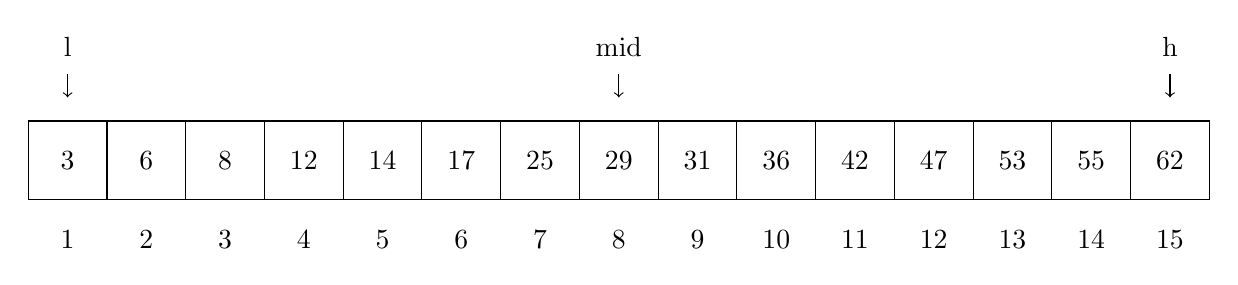
\begin{tikzpicture}
\draw (0,0) rectangle (1,1);
\draw (1,0) rectangle (2,1);
\draw (2,0) rectangle (3,1);
\draw (3,0) rectangle (4,1);
\draw (4,0) rectangle (5,1);

\draw (5,0) rectangle (6,1);
\draw (6,0) rectangle (7,1);
\draw (7,0) rectangle (8,1);
\draw (8,0) rectangle (9,1);
\draw (9,0) rectangle (10,1);

\draw (10,0) rectangle (11,1);
\draw (11,0) rectangle (12,1);
\draw (12,0) rectangle (13,1);
\draw (13,0) rectangle (14,1);
\draw (14,0) rectangle (15,1);

\node[scale=1] at (.5,0.5) {3};
\node[scale=1] at (1.5,0.5) {6};
\node[scale=1] at (2.5,0.5) {8};
\node[scale=1] at (3.5,0.5) {12};
\node[scale=1] at (4.5,0.5) {14};

\node[scale=1] at (5.5,0.5) {17};
\node[scale=1] at (6.5,0.5) {25};
\node[scale=1] at (7.5,0.5) {29};
\node[scale=1] at (8.5,0.5) {31};
\node[scale=1] at (9.5,0.5) {36};

\node[scale=1] at (10.5,0.5) {42};
\node[scale=1] at (11.5,0.5) {47};
\node[scale=1] at (12.5,0.5) {53};
\node[scale=1] at (13.5,0.5) {55};
\node[scale=1] at (14.5,0.5) {62};

\node[scale=1] at (0.5,-0.5) {1};
\node[scale=1] at (1.5,-0.5) {2};
\node[scale=1] at (2.5,-0.5) {3};
\node[scale=1] at (3.5,-0.5) {4};
\node[scale=1] at (4.5,-0.5) {5};

\node[scale=1] at (5.5,-0.5) {6};
\node[scale=1] at (6.5,-0.5) {7};
\node[scale=1] at (7.5,-0.5) {8};
\node[scale=1] at (8.5,-0.5) {9};
\node[scale=1] at (9.5,-0.5) {10};

\node[scale=1] at (10.5,-0.5) {11};
\node[scale=1] at (11.5,-0.5) {12};
\node[scale=1] at (12.5,-0.5) {13};
\node[scale=1] at (13.5,-0.5) {14};
\node[scale=1] at (14.5,-0.5) {15};

\draw [->] (0.5,1.6) -- (0.5,1.3) node[above, yshift=4mm] {l};

\draw [->] (7.5,1.6) -- (7.5,1.3) node[above, yshift=4mm] {mid};

\draw [->] (14.5,1.6) -- (14.5,1.3) node[above, yshift=4mm] {h};
\end{tikzpicture}
\end{center}


\begin{center}
\colorbox{gray!10}{\parbox{180pt}{
\begin{align*}
    \text{key } = 42
\end{align*}
}}
\end{center}


\begin{center}
  \bgroup
  \def\arraystretch{1.5}%
  \begin{tabular}{ C C C  }
    l
    &
    h
    &
    mid = $\left[ \cfrac{l+h}{2} \right]$ \vspace{5pt}
     \\ \hline
     1
     &
     15
     &
     $\cfrac{1+15}{2}$ = 8
     \\
  \end{tabular}
  \egroup
\end{center}




\vspace{30pt}



\begin{center}
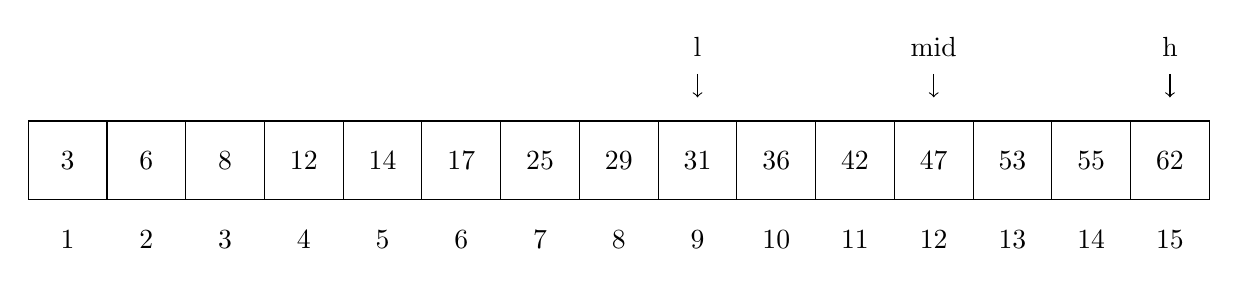
\begin{tikzpicture}
\draw (0,0) rectangle (1,1);
\draw (1,0) rectangle (2,1);
\draw (2,0) rectangle (3,1);
\draw (3,0) rectangle (4,1);
\draw (4,0) rectangle (5,1);

\draw (5,0) rectangle (6,1);
\draw (6,0) rectangle (7,1);
\draw (7,0) rectangle (8,1);
\draw (8,0) rectangle (9,1);
\draw (9,0) rectangle (10,1);

\draw (10,0) rectangle (11,1);
\draw (11,0) rectangle (12,1);
\draw (12,0) rectangle (13,1);
\draw (13,0) rectangle (14,1);
\draw (14,0) rectangle (15,1);

\node[scale=1] at (.5,0.5) {3};
\node[scale=1] at (1.5,0.5) {6};
\node[scale=1] at (2.5,0.5) {8};
\node[scale=1] at (3.5,0.5) {12};
\node[scale=1] at (4.5,0.5) {14};

\node[scale=1] at (5.5,0.5) {17};
\node[scale=1] at (6.5,0.5) {25};
\node[scale=1] at (7.5,0.5) {29};
\node[scale=1] at (8.5,0.5) {31};
\node[scale=1] at (9.5,0.5) {36};

\node[scale=1] at (10.5,0.5) {42};
\node[scale=1] at (11.5,0.5) {47};
\node[scale=1] at (12.5,0.5) {53};
\node[scale=1] at (13.5,0.5) {55};
\node[scale=1] at (14.5,0.5) {62};

\node[scale=1] at (0.5,-0.5) {1};
\node[scale=1] at (1.5,-0.5) {2};
\node[scale=1] at (2.5,-0.5) {3};
\node[scale=1] at (3.5,-0.5) {4};
\node[scale=1] at (4.5,-0.5) {5};

\node[scale=1] at (5.5,-0.5) {6};
\node[scale=1] at (6.5,-0.5) {7};
\node[scale=1] at (7.5,-0.5) {8};
\node[scale=1] at (8.5,-0.5) {9};
\node[scale=1] at (9.5,-0.5) {10};

\node[scale=1] at (10.5,-0.5) {11};
\node[scale=1] at (11.5,-0.5) {12};
\node[scale=1] at (12.5,-0.5) {13};
\node[scale=1] at (13.5,-0.5) {14};
\node[scale=1] at (14.5,-0.5) {15};

\draw [->] (8.5,1.6) -- (8.5,1.3) node[above, yshift=4mm] {l};

\draw [->] (11.5,1.6) -- (11.5,1.3) node[above, yshift=4mm] {mid};

\draw [->] (14.5,1.6) -- (14.5,1.3) node[above, yshift=4mm] {h};
\end{tikzpicture}
\end{center}







\begin{center}
  \bgroup
  \def\arraystretch{1.5}%
  \begin{tabular}{ C C C  }
    l
    &
    h
    &
    mid = $\left[ \cfrac{l+h}{2} \right]$ \vspace{5pt}
     \\ \hline
     8+1 = 9
     &
     15
     &
     $\cfrac{9+15}{2}$ = $\cfrac{24}{2}$ = 12
     \\
  \end{tabular}
  \egroup
\end{center}






\newpage








\begin{center}
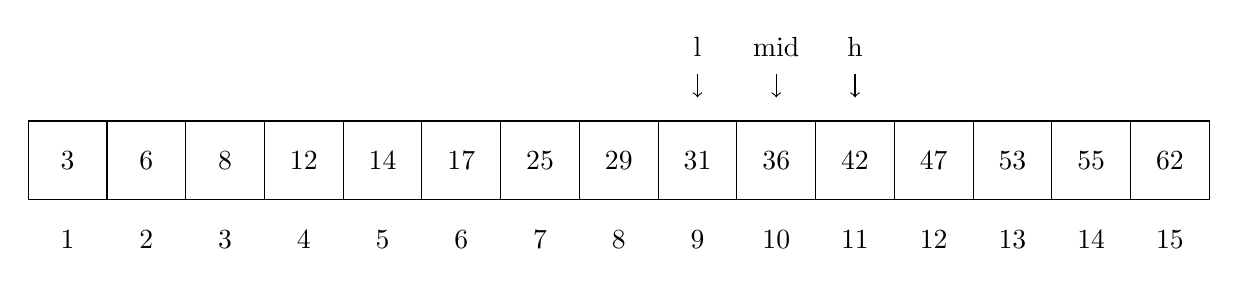
\begin{tikzpicture}
\draw (0,0) rectangle (1,1);
\draw (1,0) rectangle (2,1);
\draw (2,0) rectangle (3,1);
\draw (3,0) rectangle (4,1);
\draw (4,0) rectangle (5,1);

\draw (5,0) rectangle (6,1);
\draw (6,0) rectangle (7,1);
\draw (7,0) rectangle (8,1);
\draw (8,0) rectangle (9,1);
\draw (9,0) rectangle (10,1);

\draw (10,0) rectangle (11,1);
\draw (11,0) rectangle (12,1);
\draw (12,0) rectangle (13,1);
\draw (13,0) rectangle (14,1);
\draw (14,0) rectangle (15,1);

\node[scale=1] at (.5,0.5) {3};
\node[scale=1] at (1.5,0.5) {6};
\node[scale=1] at (2.5,0.5) {8};
\node[scale=1] at (3.5,0.5) {12};
\node[scale=1] at (4.5,0.5) {14};

\node[scale=1] at (5.5,0.5) {17};
\node[scale=1] at (6.5,0.5) {25};
\node[scale=1] at (7.5,0.5) {29};
\node[scale=1] at (8.5,0.5) {31};
\node[scale=1] at (9.5,0.5) {36};

\node[scale=1] at (10.5,0.5) {42};
\node[scale=1] at (11.5,0.5) {47};
\node[scale=1] at (12.5,0.5) {53};
\node[scale=1] at (13.5,0.5) {55};
\node[scale=1] at (14.5,0.5) {62};

\node[scale=1] at (0.5,-0.5) {1};
\node[scale=1] at (1.5,-0.5) {2};
\node[scale=1] at (2.5,-0.5) {3};
\node[scale=1] at (3.5,-0.5) {4};
\node[scale=1] at (4.5,-0.5) {5};

\node[scale=1] at (5.5,-0.5) {6};
\node[scale=1] at (6.5,-0.5) {7};
\node[scale=1] at (7.5,-0.5) {8};
\node[scale=1] at (8.5,-0.5) {9};
\node[scale=1] at (9.5,-0.5) {10};

\node[scale=1] at (10.5,-0.5) {11};
\node[scale=1] at (11.5,-0.5) {12};
\node[scale=1] at (12.5,-0.5) {13};
\node[scale=1] at (13.5,-0.5) {14};
\node[scale=1] at (14.5,-0.5) {15};

\draw [->] (8.5,1.6) -- (8.5,1.3) node[above, yshift=4mm] {l};

\draw [->] (9.5,1.6) -- (9.5,1.3) node[above, yshift=4mm] {mid};

\draw [->] (10.5,1.6) -- (10.5,1.3) node[above, yshift=4mm] {h};
\end{tikzpicture}
\end{center}







\begin{center}
  \bgroup
  \def\arraystretch{1.5}%
  \begin{tabular}{ C C C  }
    l
    &
    h
    &
    mid = $\left[ \cfrac{l+h}{2} \right]$ \vspace{5pt}
     \\ \hline
     9
     &
     12-1 = 11
     &
     $\cfrac{9+11}{2}$ = $\cfrac{20}{2}$ = 10
     \\
  \end{tabular}
  \egroup
\end{center}






\vspace{30pt}








\begin{center}
\begin{tikzpicture}
\draw (0,0) rectangle (1,1);
\draw (1,0) rectangle (2,1);
\draw (2,0) rectangle (3,1);
\draw (3,0) rectangle (4,1);
\draw (4,0) rectangle (5,1);

\draw (5,0) rectangle (6,1);
\draw (6,0) rectangle (7,1);
\draw (7,0) rectangle (8,1);
\draw (8,0) rectangle (9,1);
\draw (9,0) rectangle (10,1);

\draw (10,0) rectangle (11,1);
\draw (11,0) rectangle (12,1);
\draw (12,0) rectangle (13,1);
\draw (13,0) rectangle (14,1);
\draw (14,0) rectangle (15,1);

\node[scale=1] at (.5,0.5) {3};
\node[scale=1] at (1.5,0.5) {6};
\node[scale=1] at (2.5,0.5) {8};
\node[scale=1] at (3.5,0.5) {12};
\node[scale=1] at (4.5,0.5) {14};

\node[scale=1] at (5.5,0.5) {17};
\node[scale=1] at (6.5,0.5) {25};
\node[scale=1] at (7.5,0.5) {29};
\node[scale=1] at (8.5,0.5) {31};
\node[scale=1] at (9.5,0.5) {36};

\node[scale=1] at (10.5,0.5) {42};
\node[scale=1] at (11.5,0.5) {47};
\node[scale=1] at (12.5,0.5) {53};
\node[scale=1] at (13.5,0.5) {55};
\node[scale=1] at (14.5,0.5) {62};

\node[scale=1] at (0.5,-0.5) {1};
\node[scale=1] at (1.5,-0.5) {2};
\node[scale=1] at (2.5,-0.5) {3};
\node[scale=1] at (3.5,-0.5) {4};
\node[scale=1] at (4.5,-0.5) {5};

\node[scale=1] at (5.5,-0.5) {6};
\node[scale=1] at (6.5,-0.5) {7};
\node[scale=1] at (7.5,-0.5) {8};
\node[scale=1] at (8.5,-0.5) {9};
\node[scale=1] at (9.5,-0.5) {10};

\node[scale=1] at (10.5,-0.5) {11};
\node[scale=1] at (11.5,-0.5) {12};
\node[scale=1] at (12.5,-0.5) {13};
\node[scale=1] at (13.5,-0.5) {14};
\node[scale=1] at (14.5,-0.5) {15};

\draw [->] (10.3,1.6) -- (10.3,1.3) node[above, yshift=4mm] {l};

\draw [->] (10.5,2.8) -- (10.5,2.5) node[above, yshift=4mm] {mid};

\draw [->] (10.7,1.6) -- (10.7,1.3) node[above, yshift=4mm] {h};
\end{tikzpicture}
\end{center}







\begin{center}
  \bgroup
  \def\arraystretch{1.5}%
  \begin{tabular}{ C C C  }
    l
    &
    h
    &
    mid = $\left[ \cfrac{l+h}{2} \right]$ \vspace{5pt}
     \\ \hline
     10+1 = 11
     &
     11
     &
     $\cfrac{11+11}{2}$ = 11
     \\
  \end{tabular}
  \egroup
\end{center}





\newpage




\section{Binary Search Iterative Method}





\begin{lstlisting}[language=C++, caption=]
int BinarySearch(A,n,key) {
	l = 1;
	h = n;
	while(l <= h) {
		mid = (l+h)/2;
		if(key == A[mid]) {
			return mid;
		}
		if(key < A[mid]) {
			h = mid - 1;
		} else {
			l = mid + 1;
		}
	}
	return -1;
}
\end{lstlisting}





\newpage



\section{Binary Search Recursive Method}




\begin{lstlisting}[language=C++, caption=]
int BinarySearch(l,h,key) {
	if( l == h ) {
		if(A[l] == key) {
			return l;
		} else {
			return -1;
		}
	} else {
		mid = (l+h)/2;
		if( key == A[mid] ) {
			return mid;
		} else if( key < A[mid] ) {
			return BinarySearch(l,mid-1,key);
		} else if( key > A[mid] ) {
			return BinarySearch(mid+1,h,key)
		}
	}
}
\end{lstlisting}





\begin{align*}
T(n) = 
\begin{cases}
1 & n=1 \\
T(\frac{n}{2}) + 1 & n > 1
\end{cases}
\end{align*}

\begin{align*}
\Rightarrow f(n) = O(\log{(n)})
\end{align*}




\end{document}

